\documentclass[problem]{mcs}

\begin{pcomments}
  \pcomment{FP_college_probability}
  \pcomment{from: F03.q2, prob 5}
  \pcomment{adapted by Steven F09}
\end{pcomments}

\pkeywords{
  probability
  conditional_probability
  tree_diagram
  independence
}

%%%%%%%%%%%%%%%%%%%%%%%%%%%%%%%%%%%%%%%%%%%%%%%%%%%%%%%%%%%%%%%%%%%%%
% Problem starts here
%%%%%%%%%%%%%%%%%%%%%%%%%%%%%%%%%%%%%%%%%%%%%%%%%%%%%%%%%%%%%%%%%%%%%

\begin{problem}
Sally Smart just graduated from high school.  She was accepted to
three top colleges.

\begin{itemize}

\item With probability $4/12$, she attends Yale.

\item With probability $5/12$, she attends MIT.

\item With probability $3/12$, she attends Little Hoop Community College.

\end{itemize}

Sally will either be happy or unhappy in college.

\begin{itemize}

\item If she attends Yale, she is happy with probability $4/12$.

\item If she attends MIT, she is happy with probability $7/12$.

\item If she attends Little Hoop, she is happy with probability
$11/12$.

\end{itemize}

\bparts

\ppart[4] A tree diagram for Sally's situation is shown below.  On the
diagram, fill in the edge probabilities and at each leaf write the
probabilty of that outcome.

\vspace{0.5in}
\centerline{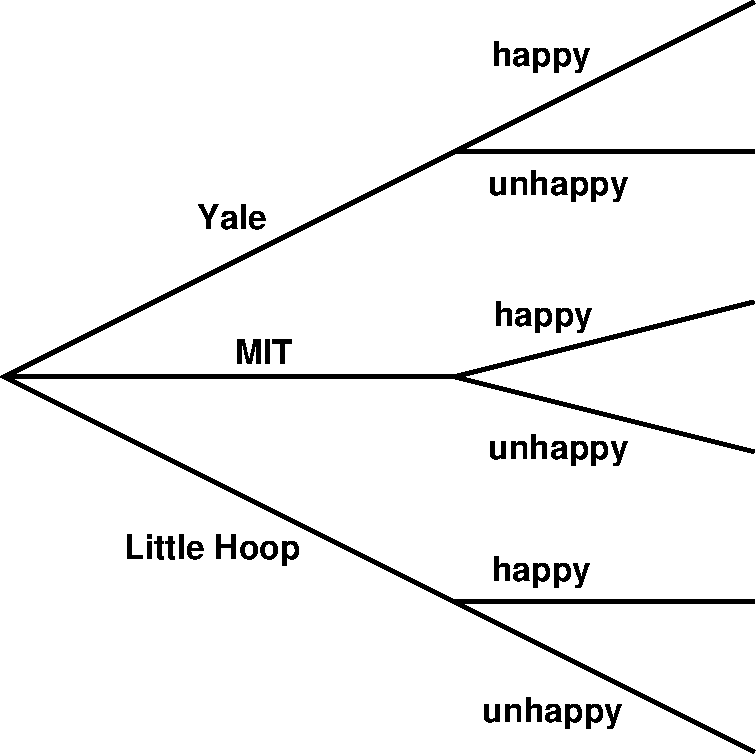
\includegraphics[height=4in]{../figures/q2-sally}}
\bigskip

\instatements{\newpage}

\ppart[4] What is the probability that Sally is happy in college?
[\vspace{2in}]

\begin{solution}
The probability that she is happy is equal to
the sum of the probabilities of the outcomes marked with an H: $16/144
+ 35/144 + 33/144 = 84/144 = 7/12$.
\end{solution}

\ppart[4] What is the probability that Sally Smart attends Yale, given
that she is happy in college?
[\vspace{2in}]

\begin{solution}
\begin{eqnarray*}
\pr{\text{attends Yale} \mid \text{happy}}
	& = & \frac{\pr{\text{attends Yale} \cap \text{happy}}}
		{\pr{\text{happy}}} \\
	& = & \frac{(4/12) \cdot (4/12)}{(7/12)} \\
	& = & 4 / 21
\end{eqnarray*}
\end{solution}

\ppart[4] Show that the event that Sally attends Yale is \textbf{not}
independent of the event that she is happy.
[\vspace{2in}]

\begin{solution}
These events are independent only if:

\begin{eqnarray}
\pr{\text{attends Yale} \mid \text{happy}} & = & \pr{\text{attends Yale}}
\end{eqnarray}

or $\pr{\text{happy}} = 0$.  However, the left side is $4/21$, the
right is $4/12$, and the probability that she is happy is nonzero
\end{solution}

\ppart[4] Show that the event that Sally Smart attends MIT \textbf{is}
independent of the event that she is happy.

\begin{solution}
These events are independent if:

\begin{eqnarray*}
\pr{\text{attends MIT}} \cdot \pr{\text{happy}}
	& = & \pr{\text{attends MIT} \cap \text{happy}}
\end{eqnarray*}

The left side is equal to $(5/12) \cdot (7/12) = 35/144$.  According
to the tree diagram, the right side is equal to $35/144$ as well.
\end{solution}

\eparts

\end{problem}

%%%%%%%%%%%%%%%%%%%%%%%%%%%%%%%%%%%%%%%%%%%%%%%%%%%%%%%%%%%%%%%%%%%%%
% Problem ends here
%%%%%%%%%%%%%%%%%%%%%%%%%%%%%%%%%%%%%%%%%%%%%%%%%%%%%%%%%%%%%%%%%%%%%
